%
% poissonverteilung.tex -- Abschnitt über Poissonverteilung in Kapitel 5
%
% (c) 2015 Prof Dr Andreas Mueller, Hochschule Rapperswil
%
\subsection{Poissonverteilung} \label{section-poissonverteilung}
\begin{figure}
\centering
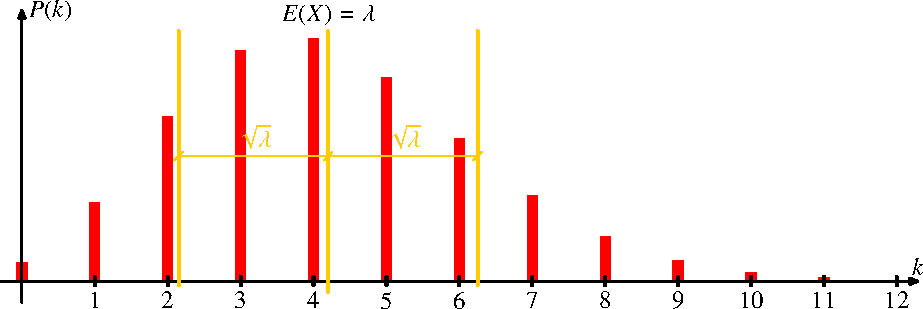
\includegraphics{images/exp-2.pdf}
\caption{Wahrscheinlichkeitsverteilung der Poisson-Verteilung für
$\lambda=4.2$, $E(X)=\lambda$ und $\operatorname{var}(X)=\sqrt{\lambda}$.
\label{poisson-verteilung}}
\end{figure}
\begin{table}
\renewcommand{\arraystretch}{1.5}
\begin{center}
\begin{tabular}{|l|l|}
\hline
Name&Poissonverteilung\\
\hline
Wahrscheinlichkeit&
\begin{minipage}{3.7in}
\vskip3pt
$\displaystyle
P_\lambda(k)=\frac{\lambda^k}{k!}e^{-\lambda}
$
\end{minipage}
\\
Erwartungswert&$\displaystyle \lambda$\\
Varianz&$\displaystyle \lambda$\\
\hline
Anwendungen&\begin{minipage}{3.7in}%
\vskip3pt
\strut
$\bullet$ Anzahl Ereignisse mit exponentialverteilten Intervallen\\
$\bullet$ Approximation der Binomialverteilung für seltene Ereignisse, die
mit Rate $\lambda$ eintreten
\strut
\end{minipage}\\[20pt]
\hline
\end{tabular}
\end{center}
\caption{Datenblatt der Poissonverteilung\label{datenblatt:poissonverteilung}}
\end{table}
Die Poissonverteilung liefert eine Antwort auf folgende Frage.
In Abschnitt
\ref{section-exponentialverteilung} wurde die Exponentialverteilung
als die Verteilung für die Ausfallwahrscheinlichkeit eines ``gedächtnislosen''
Bauteils vorgestellt.
Wir nehmen nun an, dass das Bauteil bei jedem Defekt
sofort ersetzt wird, und fragen danach, wie wahrscheinlich es ist, dass
wir in einem bestimmten Zeitintervall $k$ Ausfälle beobachten.

Sei $X_i$ die Lebensdauer des Bauteils mit der Nummer $i$, es handelt
sich dabei um eine exponentialverteilte Zufallsvariable.
Wenn im Zeitintervall
$[0,x]$ genau $k$ Ausfälle beobachtet wurden, dann heisst das, dass die
Summe von $k$ Zufallsvariablen $\le x$ ist, jene von $k+1$ Zufallsvariable
aber $>x$.
Also
\[
P(X_1+\dots+X_k\le x \wedge X_1+\dots+X_{k+1}>x)
\]
Wir berechnen diese Wahrscheinlichkeit in zwei Schritten.

Zunächst interessiert uns, wie gross die Wahrscheinlichkeit ist, dass im
Intervall $[0,x]$ mindestens $k$ Ausfälle passieren, dies ist
$P(X_1+\dots+X_k\le x)=F_{X_1+\dots+X_k}(x)$, also die Verteilungsfunktion
einer Summe von $k$ identisch exponentialverteilten Zufallsvariablen.
Wir behaupten:
\begin{satz}Sind $(X_i)_{1\le i\le k}$ identische exponentialverteilte,
unabhängige Zufallsvariablen, dann hat deren Summe folgende Verteilungsfunktion
und Wahrscheinlichkeitsdichte:
\begin{align*}
F_{X_1+\dots+X_k}(x)&=\begin{cases}
{\displaystyle 1-e^{-ax}\sum_{i=0}^{k-1}\frac{(ax)^i}{i!}}&\qquad x \ge 0\\
0&\qquad x < 0
\end{cases}
\\
\varphi_{X_1+\dots+X_k}(x)&=\begin{cases}
{\displaystyle a^k\frac{x^{k-1}}{(k-1)!}e^{-ax}}&\qquad x\ge0\\
0&\qquad x < 0\end{cases}
\end{align*}
\end{satz}
\begin{proof}[Beweis]
Wir beweisen zunächst die Formeln für die Dichtefunktion $\varphi_k$ mit
Hilfe von vollständiger Induktion.
Für $k=1$ liegt nur eine einzige
Zufallsvariable vor, durch Einsetzen von $k$ finden wir für $x>0$
\[
\varphi_1(x)=ae^{-ax},
\]
also genau die Dichte der Exponentialverteilung.
Offensichtlich ist dies die richtige Wahrscheinlichkeitsdichte.

Wir nehmen nun an, dass obige Formel die Wahrscheinlichkeitsdichte für die
Summe von $k$ Zufallsvariablen korrekt ist, und berechnen die daraus
folgende Wahrscheinlichkeitsdichte für eine Summe von $k+1$ Zufallsvariablen.
Dazu wird die Faltung verwendet, es gilt für $x>0$
\begin{align*}
\varphi_k*\varphi_1(x)
&=
\int_{-\infty}^{\infty}\varphi_k(t)\varphi_1(x-t)\,dt\\
&=\int_0^x a^k\frac{t^{k-1}}{(k-1)!}e^{-at}ae^{-a(x-t)}\,dt\\
&=a^{k+1}e^{-ax}\int_0^x \frac{t^{k-1}}{(k-1)!}\,dt\\
&=a^{k+1}e^{-ax}\left[\frac{t^k}{k!}\right]_0^x\\
&=a^{k+1}e^{-ax}\frac{x^k}{k!}=\varphi_{k+1}(x)
\end{align*}
Damit ist die Formel für $\varphi_k$ für alle $k$ gezeigt.

Aus der Wahrscheinlichkeitsdichte kann nun auch die Verteilungsfunktion
berechnet werden.
Durch partielle Integration kann man die Verteilungsfunktion
wie folgt berechnen:
\begin{align*}
F_k(x)
&=\int_0^x\varphi_k(t)\,dt\\
&=\int_0^xa^k\frac{t^{k-1}}{(k-1)!}e^{-at}\,dt\\
&=\left[-a^{k-1}\frac{t^{k-1}}{(k-1)!}e^{-at}\right]_0^x+\int_0^xa^{k-1}\frac{t^{k-2}}{(k-2)!}e^-at\,dt\\
&=-a^{k-1}\frac{x^{k-1}}{(k-1)!}e^{-ax}+F_{k-1}(x)\\
&=-\frac{(ax)^{k-1}}{(k-1)!}e^{-ax}+F_{k-1}(x)
\end{align*}
Die Verteilungsfunktion $F_1$ von $\varphi_1$ kennen wir bereits:
\[
F_1(x)=\int_0^xae^{-at}\,dt=-e^{-ax}+1.
\]
Daraus leiten wir ab
\[
F_k(x)=1-e^{-ax}\sum_{i=0}^{k-1}\frac{(ax)^i}{i!}
\]
Die Summe ist die Partialsumme für die Reihenentwicklung von $e^{ax}$,
insbesondere ist die Partialsumme immer kleiner als $a^{ax}$, also
\[
e^{-ax}\sum_{i=0}^{k-1}\frac{(ax)^i}{i!}<e^{-ax}\cdot e^{ax}=1,
\]
und damit $F_k(x) \le 0$.
Andererseits ist die Partialsumme nur ein
Polynom in $x$, welches niemals so schnell wachsen kann wie $e^{-ax}$ kleiner
wird.
Im Grenzwert $x\to\infty$ verschwindet der zweite Summand daher und
es gilt wie zu erwarten ist $\lim_{x\to\infty}F_k(x)=1$.
\end{proof}
Die hier gefundenen Verteilungen sind auch von einiger praktischer Bedeutung,
sie heissen die Erlang-Verteilungen.
\index{Erlang-Verteilung}

Um nun die Wahrscheinlichkeit $P_k(x)$ des Auftretens von genau $k$ Ausfällen
ist jetzt also die Wahrscheinlichkeit, dass bis zur Zeit $x$ mindestens
$k$ Ausfällen aufgetreten sind minus die Wahrscheinlichkeit, dass mehr
als $k$ Ausfälle aufgetreten sind: 
\[
P_k(x)=P(\text{mindestens $k$ Ausfälle})-P(\text{mehr als $k$ Ausfälle})
\]
Die Wahrscheinlichkeit von mehr als $k$ Ausfällen ist aber die Wahrscheinlichkeit
von mindestens $k+1$ Ausfällen, also
\begin{align*}
P_k(x)
&=P(\text{mindestens $k$ Ausfälle})-P(\text{mindestens $k+1$ Ausfälle})\\
&=F_k(x)-F_{k+1}(x)\\
&=1-e^{-ax}\sum_{i=0}^{k-1}\frac{(ax)^i}{i!}-1+e^{-ax}\sum_{i=0}^{k}\frac{(ax)^i}{i!}\\
&=e^{-ax}\frac{(ax)^k}{k!}
\end{align*}
Somit haben wir die Wahrscheinlichkeit berechnet, dass im betrachteten
Intervall genau $k$ Bauteile versagen.
Dies führt uns zur Definition der Poissonverteilung:
\begin{definition} Die Poissonverteilung
\[
P_\lambda(k)=\frac{\lambda^k}{k!}e^{-\lambda}
\]
beschreibt für $\lambda=ax$ die Wahrscheinlichkeit,
dass in einem Zeitintervall $[0,x]$ genau $k$ Ereignisse eintreten, wenn
die Zeit zwischen den Ereignissen exponentialverteilt ist mit Dichte
$ae^{-ax}$.
\end{definition}

\subsubsection{Erwartungswert und Varianz}
\index{Poissonverteilung!Erwartungswert}
\index{Poissonverteilung!Varianz}
\index{Erwartungswert!Poissonverteilung}
\index{Varianz!Poissonverteilung}
Mit Hilfe der geschlossenen Formel für die Poissonverteilung kann man
jetzt auch Erwartungswert und Varianz berechnen:
\begin{align*}
E(X)
&=\sum_{k=0}^\infty kP_\lambda(k)\\
&=\sum_{k=0}^\infty k\frac{\lambda^k}{k!}e^{-\lambda}\\
&=\lambda e^{-\lambda}\sum_{k=1}^\infty\frac{\lambda^{k-1}}{(k-1)!}\\
&=\lambda e^{-\lambda}\sum_{k=0}^\infty\frac{\lambda^k}{k!}\\
&=\lambda e^{-\lambda}e^\lambda=\lambda\\
\end{align*}
Für $E(X^2)$ finden wir analog
\begin{align*}
E(X^2)
&=\sum_{k=0}^\infty k^2P_\lambda(k)\\
&=\sum_{k=0}^\infty k^2\frac{\lambda^k}{k!}e^{-\lambda}\\
&=\lambda e^{-\lambda}\sum_{k=1}^\infty k\frac{\lambda^{k-1}}{(k-1)!}\\
&=\lambda e^{-\lambda}\frac{d}{d\lambda}\sum_{k=1}^\infty \frac{\lambda^k}{(k-1)!}\\
&=\lambda e^{-\lambda}\frac{d}{d\lambda}\lambda\sum_{k=1}^\infty \frac{\lambda^{k-1}}{(k-1)!}\\
&=\lambda e^{-\lambda}\frac{d}{d\lambda}\lambda e^{\lambda}\\
&=\lambda e^{-\lambda}(e^\lambda+\lambda e^\lambda)\\
&=\lambda(1+\lambda)
\end{align*}
Daraus erhalten wir die Varianz:
\[
\operatorname{var}(X)=E(X^2)-E(X)^2=\lambda^2+\lambda -\lambda^2 =\lambda.
\]
\begin{satz}
Die Poissonverteilung $P\lambda(k)$ hat Erwartungswert
$E(X)=\lambda$ und Varianz $\operatorname{var}(X)=\lambda$.
\end{satz}

\subsubsection{Poissonverteilung als Approximation für die Binomialverteilung}
\index{Poissonverteilung!Approximation der Binomialverteilung}
Das folgende Experiment soll diese Anwendung motivieren: 18 mal werden zwei 
Würfel geworfen, und in einem $6\times 6$-Feld das Feld mit der
erwürfelten Zeilen- und Spalten-Nummer angekreuzt.
Dabei muss man darauf
achten, immer den gleichen Würfel für die Zeilen-Nummern zu verwenden.
Dann wird ausgezählt, wie viele Felder $k=0$, $k=1$, $k=2$,\dots\ Kreuze
enthalten.

Natürlich ist dies ein Bernoulli-Experiment.
Die Wahrscheinlichkeit, ein
bestimmtes Feld anzukreuzen, ist $p=\frac{1}{36}$, das Experiment
wird $18$ mal wiederholt.
Die Wahrscheinlichkeit $P(k)$, dass das Feld $k$ mal
angekreuzt wurde, ist durch die Binomialverteilung gegeben:
\[
P(k)=\binom{n}{k}p^k(1-p)^{n-k}.
\]

Leider ist dieser Ausdruck für grosses $n$ schwierig auszurechnen.
Wir suchen also nach einer Approximation, die leichter auszuwerten ist.
Dabei können wir nicht einfach $n\to\infty$ gehen lassen, denn die
Wahrscheinlichkeit $P(k)$ würde dann auch anwachsen.
Wir müssen
gleichzeitig die Wahrscheinlichkeit kleiner machen, so dass die Rate $\lambda$,
mit der Kreuze gemacht werden, gleich bleibt.
Im Experiment wird
die Hälfte ($\lambda=\frac{18}{36}=\frac12$) der Felder angekreuzt.
Die Wahrscheinlichkeit $p$ muss also mit $\lambda$ über die Formel
\[
p=\frac{\lambda}{n}
\]
zusammenhängen.

\begin{figure}
\begin{center}
\begin{tabular}{|r|r|r|r|r|}
\hline
$k$&Binomial&empirisch&Poisson&\\
\hline
0&   0.60440867 & 0.60226943 & 0.60653066 & 21.8351 \\
1&   0.30646073 & 0.30971007 & 0.30326533 & 10.9176 \\
2&   0.07553610 & 0.07521756 & 0.07581633 &  2.7294 \\
3&   0.01205740 & 0.01146811 & 0.01263606 &  0.4549 \\
4&   0.00140104 & 0.00123035 & 0.00157951 &  0.0569 \\
5&   0.00012629 & 0.00009816 & 0.00015795 &  0.0057 \\
6&   0.00000919 & 0.00000599 & 0.00001316 &  0.0005 \\
7&   0.00000055 & 0.00000031 & 0.00000094 &  0.0000 \\
8&   0.00000003 & 0.00000002 & 0.00000006 &  0.0000 \\
9&   0.00000000 & 0.00000000 & 0.00000000 &  0.0000 \\
\hline
\end{tabular}
\end{center}
\caption{Wahrscheinlichkeit, in einem $6\times 6$-Feld nach 18-maligem
zufälligem Ankreuzen eines Feldes gefunden Verteilung der Anzahl Kreuze.
Die Spalte ganz rechts enthält die erwartet Anzahl Felder mit $k$ Kreuzen.
\label{cross36}}
\end{figure}

Damit kann man jetzt die Approximation durchführen:
\begin{align*}
\binom{n}{k}p^k(1-p)^{n-k}
&=
\frac{n(n-1)(n-2)\dots(n-k+1)}{k!}\cdot \biggl(\frac{\lambda}n\biggr)^k\cdot \biggl(1-\frac{\lambda}n\biggr)^{n-k}\\
&=
\frac{\lambda^k}{k!}
\cdot\frac{n}{n}
\cdot\frac{n-1}{n}
\cdot\frac{n-2}{n}
\dots
\cdot\frac{n-k+1}{n}
\cdot
\biggl(1-\frac{\lambda}n\biggr)^n
\cdot
\biggl(1-\frac{\lambda}n\biggr)^{-k}
\end{align*}
Für $n\to\infty$ strebt der letzte Term gegen $1$.
Der zweitletzte Term strebt gegen $e^{-\lambda}$.
Jeder der Faktoren $\frac{n-i}n$ strebt gegeben $1$, und es sind ja nur
$k$ solche Faktoren, $k$ bleibt während des Grenzübergangs unverändert.
Daraus leiten wir ab:
\[
\lim_{n\to\infty} 
\binom{n}{k}p^k(1-p)^{n-k}
=
\frac{\lambda^k}{k!}e^{-\lambda}=P_{\lambda}(k),
\]
die Poisson-Verteilung zum Parameter $\lambda$.

Wenden wir dies auf das ursprüngliche Experiment an, also $n=36$,
$\lambda=0.5$, finden wir die Resultate in Tabelle~\ref{cross36}. 
Die Abweichungen in der Spalte der empirischen Resultate kommt übrigens
nicht daher, dass zu wenige Versuch gemacht worden wären, sondern daher,
dass wir jeweils immer alle Felder ausgezählt haben.
Diese sind aber nicht
unabhängig.
Die beim Auszählen des $6\times 6$-Feldes gefundenen Werte
sind also gar nicht die Resultate von $n$ unabhängigen Bernoulli-Experimenten.
